\documentclass[final,hyperref={pdfpagelabels=false}]{beamer}
\usepackage{grffile}
\mode<presentation>{\usetheme{I6pd2}}
\usepackage[english]{babel}
\usepackage[latin1]{inputenc}
\usepackage{amsmath,amsthm, amssymb, latexsym}
\usepackage{tikz}
\usetikzlibrary{shapes.geometric, arrows,backgrounds,fit}
\usepackage{booktabs}
\usepackage{caption}
\captionsetup{justification={justified}}
\usepackage[square,numbers]{natbib}
\usepackage{ragged2e}
\tikzstyle{arrow} = [thick,line width=0.8mm,->,>=stealth]
\usepackage{hyperref}

%\usepackage{times}\usefonttheme{professionalfonts}  % obsolete
%\usefonttheme[onlymath]{serif}
\boldmath
\usepackage[orientation=portrait,size=a0,scale=1.4,debug]{beamerposter}
% change list indention level
% \setdefaultleftmargin{3em}{}{}{}{}{}


%\usepackage{snapshot} % will write a .dep file with all dependencies, allows for easy bundling

\usepackage{array,booktabs,tabularx}
\newcolumntype{Z}{>{\centering\arraybackslash}X} % centered tabularx columns
\newcommand{\pphantom}{\textcolor{ta3aluminium}} % phantom introduces a vertical space in p formatted table columns??!!
\setbeamercolor{background canvas}{bg=lightgray}
\setbeamercolor*{block body}{bg=white, fg=black}
\listfiles
%%%%%%%%%%%%%%%%%%%%%%%%%%%%%%%%%%%%%%%%%%%%%%%%%%%%%%%%%%%%%%%%%%%%%%%%%%%%%%%%%%%%%%
\graphicspath{{figures/}}
 
\title{
\huge Collaborative Text Filtering}
\author{Peter J. Bakke, Daniel Horvath, Christian Hansen and Thomas Brenner}
\institute[Department]{\small DTU Compute, Technical University of Denmark}
\date[December. 17th, 2018]{December. 17th, 2018}

%%%%%%%%%%%%%%%%%%%%%%%%%%%%%%%%%%%%%%%%%%%%%%%%%%%%%%%%%%%%%%%%%%%%%%%%%%%%%%%%%%%%%%
\newlength{\columnheight}
\setlength{\columnheight}{105cm}

\begin{document}

\begin{frame}
 \begin{columns}
% ---------------------------------------------------------%
% Set up  COLUMN 1
% ---------------------------------------------------------%
 \begin{column}{.49\paperwidth}
 \begin{beamercolorbox}[center,wd=\textwidth]{postercolumn}
 \begin{minipage}[T]{.99\textwidth}  % tweaks the width, makes a new \textwidth
 \parbox[t][\columnheight]{\textwidth}{ % must be some better way to set the the height, width and textwidth simultaneously
                                                            % Since all columns are the same length, it is all nice and tidy.  You have to get the height empirically

% ---------------------------------------------------------%
% set up block  INTRODUCTION
% ---------------------------------------------------------%
\begin{block}{Introduction}
 \begin{columns}
 \begin{column}{1\textwidth}


%\begin{minipage}[t]{.45\textwidth}
%
%\begin{figure}
% \centering
% \includegraphics[width=\linewidth]{figures/pep_MHCII.pdf}
%\caption{MHCII molecules present peptides derived from the extracellular to T-helper cells. Here we predict which peptides are able to bind a given MHCII molecule, which is an important step on the way to identifying T-cell epitopes.}
%\end{figure} 			
%
%\end{minipage} \hspace{1cm} \begin{minipage}[t]{.45\textwidth}
\centering
\begin{minipage}[t]{0.98\textwidth}

\small{Collaborative text filtering is one of the most popular and effective approaches for recommender systems. Recommender systems are based on the idea, that given previously collected data about users and their interactions with items, you can predict whether a given user wants to have an interaction with a given item. This is widely used for platforms like Netflix, Amazon, Youtube and news websites. These platforms can increase their profits by being able to predict their consumers interests and showing content relevant for the user. 

The purpose of this project is to match two text descriptions of varied lengths. More concretely job applications with job descriptions. The hope is of course, to have a model that matches job applicants with open job positions.
\vspace{0.5cm}
}



\end{minipage} \hspace{1cm}


      
\end{column}
 \end{columns}
 \end{block}
 \vfill


% ---------------------------------------------------------%
% set up block  DATA
% ---------------------------------------------------------%

 \begin{block}{Data}
 \begin{columns}
 \begin{column}{1\textwidth}
 


\vspace{-0.5cm}

\begin{minipage}[t]{0.98\textwidth}
\begin{itemize}
\justifying
\small{
        \item We use the publicly available \textbf{MovieLens} dataset from \url{https://grouplens.org/datasets/movielens/} for the first part of our project
	\item We use the publicly available \textbf{CiteULike} from \url{http://www.citeulike.org/faq/data.adp} for the second part of our project
	\item We use a private dataset called \textbf{TalentFox} for the final part of our project
}
\end{itemize}


\end{minipage} 
%\end{minipage} \hspace{1cm} \begin{minipage}[t]{.5\textwidth}


\vspace{0.5cm}

					
          
\end{column}
\end{columns}
\vskip-1ex
\end{block}
\vfill

% ---------------------------------------------------------%
% set up block  DATA
% ---------------------------------------------------------%

 \begin{block}{Key points}
 \begin{columns}
 \begin{column}{1\textwidth}
 


\vspace{-0.5cm}

\begin{minipage}[t]{0.98\textwidth}
\begin{itemize}
\justifying
\small{
        \item We construct a baseline model using \textbf{Matrix Factorization} on the MovieLens, CiteUlike, and TalentFox data
	\item We construct a \textbf{Collaborative Text Filtering} model on the same data 
	using
	{\setbeamertemplate{itemize items}[ball]
	\begin{itemize}
	\small{
	\item  \quad Feed Forward Networks 
	\item  \quad LSTM Networks}
	\end{itemize}}
	And compare the results to the baseline model
	\item We implement the models using the \textbf{Pytorch} deep learning framework and \textbf{TorchText}
	\item We train the models on the \textbf{Google Colab} GPU cloud
}
\end{itemize}


\end{minipage} 
%\end{minipage} \hspace{1cm} \begin{minipage}[t]{.5\textwidth}


\vspace{0.5cm}

					
          
\end{column}
\end{columns}
\vskip-1ex
\end{block}
\vfill




% ---------------------------------------------------------%
% set up block  MovieLens
% ---------------------------------------------------------%


 \begin{block}{MovieLens}
 \begin{columns}
 \begin{column}{1\textwidth}


%\vspace{0.5cm}

\centering
\begin{minipage}[t]{0.96\textwidth}
			

\hspace{0.5cm} 
\vspace{-1cm}
\begin{columns}
 \begin{column}{0.45\textwidth}
 \justifying
 \small{
	The MoveieLens dataset consist of 20 million ratings on a scale from 1 to 5, of 27,000 different movies by 138,000 users. Taking outset in the MovieLens dataset the objective is to predict how a specific user will rate a specific movie. }
 \end{column}
 \begin{column}{0.49\textwidth}

\begin{table}[h]
\small
\centering
\caption{Results} 
\label{res:MovieLens_results}
\begin{tabular}{llllll}
\toprule
Model  & Best accuracy        & Best Epoch     & Something else    \\
\midrule
MF  	&  0.1337        & 2       & 0.1337    \\
FNN	  &  0.1337        & 12      & 0.1337    \\
\bottomrule
\end{tabular}
\end{table}

 \end{column}
 \end{columns}
 
 \begin{figure}

\includegraphics[width=0.85\textwidth]{movielensnet.png}
 \caption{MovieLens neural net representation}
\end{figure}  

\end{minipage}



\vspace{0.5cm}

					
                  
\end{column}
\end{columns}
\vskip-1ex
\end{block}
\vfill


% ---------------------------------------------------------%
% set up block  MovieLens
% ---------------------------------------------------------%


 \begin{block}{CiteULike}
 \begin{columns}
 \begin{column}{1\textwidth}


%\vspace{0.5cm}

\centering
\begin{minipage}[t]{0.96\textwidth}
			

\hspace{0.5cm} 
\vspace{-1cm}
\begin{columns}
 \begin{column}{0.45\textwidth}
 \justifying
 \small{
	The CiteULike dataset consist of users that have marked that they have read different scientific articles. In total we have approximately 200k articles spread across approximately 5500 users Taking outset in the CiteULike dataset the objective is to predict whether a specific reader is interested in an article. }
 \end{column}
 \begin{column}{0.49\textwidth}

\begin{table}[h]
\small
\centering
\caption{Results} 
\label{res:CiteULike_results}
\begin{tabular}{llllll}
\toprule
Model  & Best accuracy        & Best Epoch     & Something else    \\
\midrule
MF  	&  0.1337        & 2       & 0.1337    \\
FNN	  &  0.1337        & 12      & 0.1337    \\
LSTM	&  0.1337        & 24      & 0.1337    \\
\bottomrule
\end{tabular}
\end{table}

 \end{column}
 \end{columns}
 
 \begin{figure}

\includegraphics[width=0.85\textwidth]{movielensnet.png}
 \caption{Need to draw the LSTM net}
\end{figure}  

\end{minipage}



\vspace{0.5cm}

					
                  
\end{column}
\end{columns}
\vskip-1ex
\end{block}
\vfill


% ---------------------------------------------------------%
% set up block REFERENCES
% ---------------------------------------------------------%



}
\end{minipage}
\end{beamercolorbox}
\end{column}
% ---------------------------------------------------------%
% end the COLUMN 1
% ---------------------------------------------------------%
 

% ---------------------------------------------------------%
% Set up COLUMN 2
% ---------------------------------------------------------%
    
\begin{column}{.49\paperwidth}
\begin{beamercolorbox}[center,wd=\textwidth]{postercolumn}
\begin{minipage}[T]{.99\textwidth} % tweaks the width, makes a new \textwidth
\parbox[t][\columnheight]{\textwidth}{ % must be some better way to set the the height, width and textwidth simultaneously
            											% Since all columns are the same length, it is all nice and tidy.  You have to get the height empirically
            
% ---------------------------------------------------------%
% set up block RESULTS + DISCUSSION
% ---------------------------------------------------------%

% ---------------------------------------------------------%
% set up block  MovieLens
% ---------------------------------------------------------%


 \begin{block}{TalentFox}
 \begin{columns}
 \begin{column}{1\textwidth}


%\vspace{0.5cm}

\centering
\begin{minipage}[t]{0.96\textwidth}
			

\hspace{0.5cm} 
\vspace{-1cm}
\begin{columns}
 \begin{column}{0.45\textwidth}
 \justifying
 \small{
	The TalentFox dataset consist of job applicants and job descriptions. The modelling aim is to find the best suited candidate for a specific job description }
 \end{column}
 \begin{column}{0.49\textwidth}

\begin{table}[h]
\small
\centering
\caption{Results} 
\label{res:TalentFox_results}
\begin{tabular}{llllll}
\toprule
Model  & Best accuracy        & Best Epoch     & Something else    \\
\midrule
MF  	&  0.1337        & 2       & 0.1337    \\
FNN	  &  0.1337        & 12      & 0.1337    \\
LSTM	&  0.1337        & 24      & 0.1337    \\
\bottomrule
\end{tabular}
\end{table}

 \end{column}
 \end{columns}
 
 \begin{figure}

\includegraphics[width=0.85\textwidth]{movielensnet.png}
 \caption{Need to draw another diagram here}
\end{figure}  

\end{minipage}



\vspace{0.5cm}

					
                  
\end{column}
\end{columns}
\vskip-1ex
\end{block}
\vfill

\begin{block}{Comparison of results}

\begin{columns}
\begin{column}{1\textwidth}

\centering

%\vspace{2.5cm}
\centering
\begin{minipage}[t]{.95\textwidth}


\vspace{-1cm}
\begin{table}[h]
\small
\caption{Confusion matrix of the test set on the final DeepLoc model using profiles encoding. Sens. = Sensitivity, MCC = Matthews Correlation Coefficient}
\begin{tabular}{p{8cm}p{2cm}p{2cm}p{2cm}p{2cm}p{2cm}p{2cm}p{2cm}p{2cm}p{2cm}p{2cm}p{2.5cm}p{2.5cm}}
\toprule
Location      & \multicolumn{10}{l}{Number of predicted proteins}        & Sens. & MCC \\
\midrule
Nucleus          & 680 & 103 & 4   & 5   & 2   & 8   & 1   & 2  & 2 & 1 & 0.842 & 0.784 \\
Cytoplasm         & 94  & 361 &  7  & 18  & 5   & 4   & 3   & 8  & 1 & 7 & 0.711 & 0.608 \\
Extracellular    & 3   & 5   & 365 &  5  & 5   & 4   & 2   & 0  & 4 & 0 & 0.929 & 0.907 \\
Mitochondrion     & 9   & 21  & 0   & 247 &  0  & 5   & 14  & 2  & 1 & 3 & 0.818 & 0.812 \\
Cell membrane     & 5   & 15  & 6   & 1   & 203 & 20  & 1   & 4  & 18& 0 & 0.744 & 0.732 \\
Endoplasmic ret.               & 3   & 6   & 6   & 3   & 18  & 120 &  1  & 7  & 8 & 1 & 0.694 & 0.654 \\
Plastid           & 1   & 2   & 0   & 8   & 0   & 0   & 140 &  0 & 1 & 0 & 0.921 & 0.883 \\
Golgi apparatus  & 4   & 17  & 1   & 0   & 9   & 8   & 1   & 26 & 4 & 0 & 0.371 & 0.414 \\
Lysosome/Vacuole & 0   & 7   & 11  & 1   & 20  & 9   & 0   & 4  & 12& 0 & 0.188 & 0.194 \\
Peroxisome       & 0   & 13  & 0   & 4   & 1   & 4   & 0   & 0  & 0 & 8 & 0.267 & 0.321 \\
\bottomrule

\end{tabular}
\end{table}


\end{minipage}

\end{column}
\end{columns}
\end{block}

\vfill

\begin{block}{More results}

\begin{columns}
\begin{column}{1\textwidth}

\centering

%\vspace{2.5cm}
\centering
\begin{minipage}[t]{.95\textwidth}


\vspace{-0.5cm}

\small{We are able to represent what regions in the sequence are relevant for each subcellular localization to perform the prediction.}

\vspace{0.4cm}
\begin{figure}
\centering
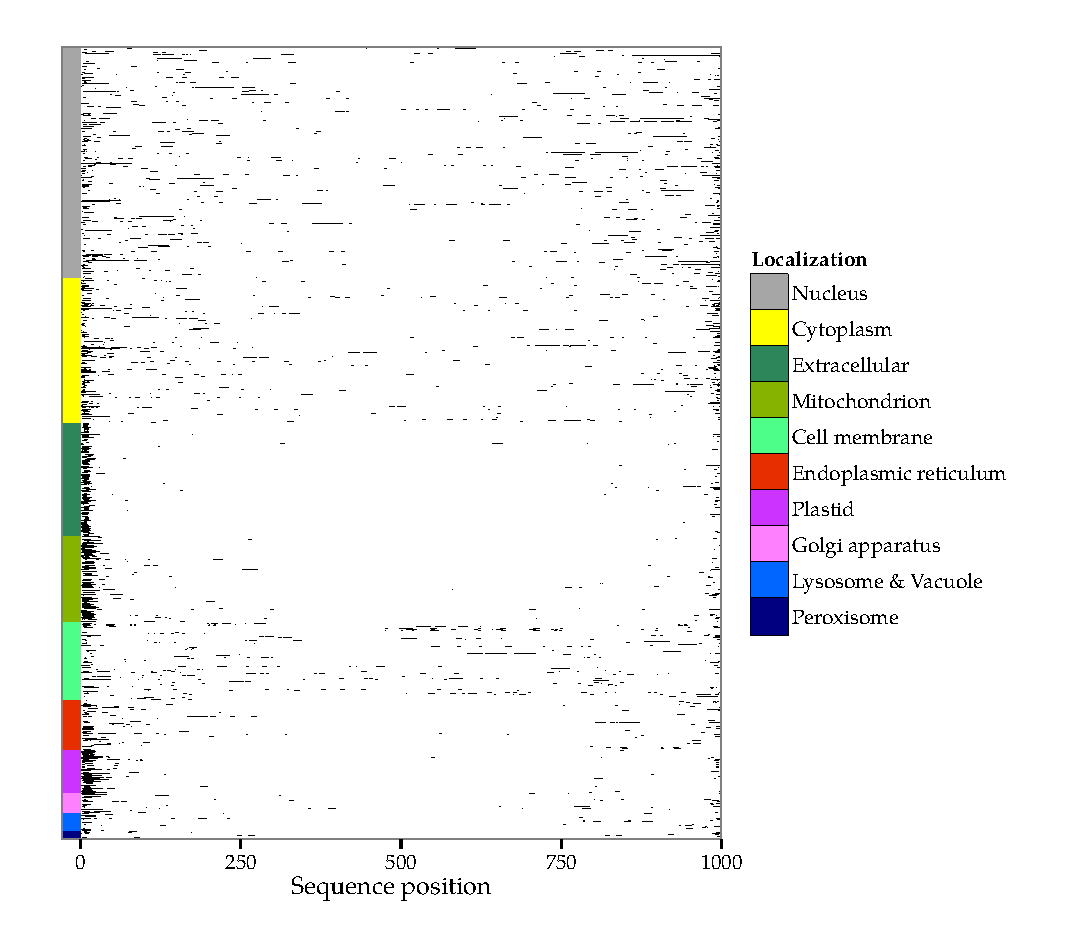
\includegraphics[width=0.9\linewidth]{Sequence_importance.eps}
 \caption{Sequence importance across the protein sequence of DeepLoc test set when making the prediction.}
\end{figure}  


\end{minipage}

\end{column}
\end{columns}
\end{block}	

\vfill

\begin{block}{Acknowledgements}
\centering
\begin{minipage}[t]{0.98\textwidth}

\small{The authors wish to thank Alexander R. Johansen and Jose Juan Almagro Armenteros from DTU Lyngby for their constructive feedback and fruitful discussions during the process of the project.}
\end{minipage}
\end{block}
\vfill
\begin{block}{References}

{\footnotesize
\bibliographystyle{abbrvnat}	
\bibliography{biblio}
}			
\end{block}
\vfill


         
}
\end{minipage}
\end{beamercolorbox}
\end{column}
\end{columns}	
% ---------------------------------------------------------%
% end the COLUMN 2
% ---------------------------------------------------------%
  
  
\vskip1ex
%\tiny\hfill\textcolor{ta2gray}{Created with \LaTeX \texttt{beamerposter}  \url{http://www-i6.informatik.rwth-aachen.de/~dreuw/latexbeamerposter.php}}
\tiny\hfill{Created with \LaTeX \texttt{beamerposter}  \url{http://www-i6.informatik.rwth-aachen.de/~dreuw/latexbeamerposter.php} \hskip1em}
\end{frame}
\end{document}